\documentclass{beamer}
%
% Choose how your presentation looks.
%
% For more themes, color themes and font themes, see:
% http://deic.uab.es/~iblanes/beamer_gallery/index_by_theme.html
%
\mode<presentation>
{
  \usetheme{default}      % or try Darmstadt, Madrid, Warsaw, ...
  \usecolortheme{default} % or try albatross, beaver, crane, ...
  \usefonttheme{default}  % or try serif, structurebold, ...
  \setbeamertemplate{navigation symbols}{}
  \setbeamertemplate{caption}[numbered]
} 
\usepackage[english]{babel}
\usepackage[utf8x]{inputenc}
\usepackage{verbatim}
\usepackage{tikz}
\usepackage{algorithm}
\usepackage{algpseudocode}
\usepackage{subfig}
\usepackage{gensymb}
\usetikzlibrary{calc}
\usetikzlibrary{plotmarks}
\usetikzlibrary{shapes}
\usetikzlibrary{arrows}
\usetikzlibrary{positioning}

\renewcommand{\vec}[1]{
    \boldsymbol{#1}
}

\newcommand{\uvec}[1]{
    \boldsymbol{\hat{#1}}
}

\newcommand{\Arg}[1]{
    \mathrm{Arg}~#1
}

\DeclareMathOperator*{\argmax}{arg\,\text{max}}
\DeclareMathOperator*{\argmin}{arg\,\text{min}}

\newcommand{\Drone}[3]{
  \draw[
    fill=gray,
    rounded corners=1mm,
    rotate around={#3:(#1,#2)}
  ] (#1,#2) --++ (-.5,.35) --++ (0.25,-.35) --++ (-0.25,-.35) -- (#1,#2);
}

\tikzstyle{point} = [
  circle,
  minimum width=3.5pt,
  inner sep=0,
  fill=black
]

\tikzstyle{my_v} = [
  ->,
  line width = 1.2pt
]

\tikzstyle{block} = [rectangle, draw, fill=blue!20, 
text width=5em, text centered, rounded corners, minimum height=4em]
\tikzstyle{line} = [draw, -latex']

\title{Robust autonomous landing of fixed-wing UAVs in wind}
\institute{Half time report}
\author{Tobias Fridén}
\date{14/11 - 2019}

\begin{document}

\begin{frame}
    \titlepage
\end{frame}

\section{Problem description}

\begin{frame}{Problem description}
Research questions:
\begin{enumerate}
    \item How can sampling-based motion planning techniques be used to generate landing sequences for fixed-wing UAVs?
    \item How can safe landings!!! be guaranteed when taking wind effects into account?
\end{enumerate}
\end{frame}

\begin{frame}{Scope}
    \begin{figure}
        \begin{center}
            \resizebox{\linewidth}{!}{
                \begin{tikzpicture}[node distance = 3cm, auto]
                    \node[block] (init){Behaviour layer};
                    \node[block, dashed, below of=init] (user){User};
                    \node[block, right of=init] (mp){Motion planning};
                    \node[block, right of=mp] (ctrl){Tracking controllers};
                    \node[block, right of=ctrl] (uav){\ac{UAV}};
        
                    \path[line] (user) -> node[midway, left]{Manual input} (init);
                    \path[line] (init) -> node[midway, above, align=left, yshift=.9cm]{High-level \\ commands} (mp);
                    \path[line] (mp) -> node[midway, above, align=left, yshift=.9cm]{Reference \\ trajectory} (ctrl);
                    \path[line] (ctrl) -> node[midway, above, align=left, yshift=.9cm]{Actuator \\ outputs} (uav);
                \end{tikzpicture}
            }
        \end{center}
        \caption{Components of a general autonomous system}
        \label{fig:autonomous}
    \end{figure}
\end{frame}

\section{Theory}

\begin{frame}{Kinematic model}
    \begin{align}\label{eq:traj_model}
        \dot{x}_N &= \airspd\cos\psi + \windspd\cos\winddir \\
        \dot{y}_E &= \airspd\sin\psi + \windspd\sin\winddir \\
        \dot{\psi} &= \frac{g}{\airspd}\tan\phi
    \end{align}
    \begin{align}
        \dot{\phi} = f_\phi(\phi-\phi^c)
    \end{align}
\end{frame}

\begin{frame}{Straight path following in wind}
    \begin{figure}
        \begin{center}
            \resizebox{.3\linewidth}{!}{
                \tikzstyle{myaxis}=[
                    ->,
                    line width=1pt
                    ]
                    \begin{tikzpicture}
                        \Drone{2}{1}{65}
                        \coordinate (test) at (50:2);
                        \draw[myaxis] (0, 0) -- node[at end, left]{$x_N$} (0, 2);
                        \draw[myaxis] (0,0) -- node[at end, below]{$y_E$} (2, 0);
        
                        \draw[myaxis] (0, 0) -- node[at end, left]{$p_{N,s}$} (test);
                        \draw[myaxis] (0,0) -- node[at end, below]{$p_{E,s}$} (-40:2);
                        \draw[myaxis](0,0.75) arc(90:50:0.75) node[midway, above]{$\psi_s$};
                        \draw[dashed](0, 0) -- (50:4);
                        \draw[dashed](2,1) -- node[midway, anchor=south west]{$d$} (test);
                    \end{tikzpicture}      
            }
        \end{center}
        \caption{Coordinate frame for straight path following}
        \label{fig:coord_straight}
    \end{figure}
\end{frame}

\begin{frame}{Straight path following in wind (contd)}
    \begin{align}
        \dot{d}\equiv\dot{p}_{E,s} &= \airspd\sin(\psi-\psi_s) + \windspd\sin(\winddir-\psi_s)\\
        \dot{\psi} &= \frac{g}{\airspd}\tan\phi
    \end{align}
    $d\approx0$, $\dot{d}\approx0$ means that $\airspd\sin(\psi-\psi_s) + \windspd\sin(\winddir-\psi_s)=0$ so 
    \begin{equation}\label{eq:wca}
        \wca\equiv-\arcsin\left(\frac{\windspd}{\airspd}\sin(\winddir-\psi_s)\right) + \psi_s
    \end{equation}
\end{frame}

\begin{frame}{Trajectory following controller}
    \begin{figure}[htb]
        \begin{center}
        \tikzstyle{point} = [
            circle,
            minimum width=3.5pt,
            inner sep=0,
            fill=black
        ]
        \tikzstyle{my_v} = [
            ->,
            line width = 1.2pt
        ]
        \resizebox{.7\linewidth}{!}{
            \begin{tikzpicture}[scale=0.85]
                %\draw[help lines](0,0) grid (10,10);
                \coordinate (origin) at (1,1);
                \coordinate (drone) at (2,6);
                \coordinate (goal) at (9,9);
                \coordinate (ref) at (7,7);
                
                \node[anchor=300] at (drone) {$\vec{p}$};
                \draw[my_v] (drone) -- node[above, near end, anchor=south east]{$\vel$} ++ ({atan(2)}:2.5);
        
                \draw[->] (drone) -- node[right, at end]{$a^c$}++ (-45:1);

                \draw[->] ([yshift=0.7cm]drone) arc(90:{atan(2)}:0.7) node[above,midway]{$\psi$};
                \draw[dashed] (drone) --++ (0,1);
                \draw[->] (drone) ++ (0.5,1) arc({atan(2)}:{atan(0.2)}:{sqrt(1.25)}) node[midway,anchor=223]{$\eta$};
                
                \node[anchor=north west] at (origin) {$\vec{p}_s$};
        
                \node[anchor=north west] at (goal) {$\vec{p}_g$};
                
                \draw (drone) -- node[above,sloped]{$L_1$} (ref);
                \node[point] at (ref) {};
                \node[anchor=north west] at (ref) {$P$};
                
                \draw[] (origin) -- node[above, at end]{} (goal);
                \node[point] at (origin) {};
                \node[point] at (goal) {};
                \node[point] at (drone) {};
            
                \Drone{2}{6}{70};
        
            \end{tikzpicture}
        }  
        \caption{$L_1$ controller logic}
        \label{fig:ss_defs}
        \end{center}
    \end{figure}
\end{frame}

\begin{frame}{Trajectory following controller (contd)}
    \begin{equation}
        \vel = \airspd\begin{bmatrix}
            \cos\psi \\
            \sin\psi
        \end{bmatrix}
        + \windspd\begin{bmatrix}
            \cos\winddir\\
            \sin\winddir
        \end{bmatrix}
    \end{equation}
    \begin{equation}\label{eq:lat_acc}
        a^{c}=2\frac{V^2}{L_1}\sin\eta, \quad V=\|\vel\|
    \end{equation}
    \begin{equation}\label{eq:roll_cmd}
        \phi^{c}=\tan^{-1}(a^{c}/g)
    \end{equation}
\end{frame}

\section{Motion planning}
\begin{frame}{State and action set definitions}
    \begin{equation}
        x=(x_N, y_E, \psi)
    \end{equation}
    \begin{equation}
        u=(p_{N,g}, p_{E,g})
    \end{equation}
\end{frame}

\begin{frame}{Closed loop system}
    \eqref{eq:traj_model} + \eqref{eq:roll_cmd} $\Rightarrow$
    \begin{equation}
        \dot{\psi}=\frac{a^c(x, u)}{\airspd}
    \end{equation}
    Physical constraint: $\dot{\psi}\leq\dot{\psi}_{\text{max}}$ $\Rightarrow$
    \begin{equation}\label{eq:saturation}
        \underline{\dot{\psi}}(x, u)=\begin{cases}
            a^c(x, u)/\airspd & |a^c(x, u)/\airspd| \leq \dot{\psi}_{\text{max}} \\
            \text{sgn}(a^c(x, u)/\airspd)\dot{\psi}_{\text{max}} & \text{otherwise}
        \end{cases}
    \end{equation}
\end{frame}

\begin{frame}{Closed loop system (contd)}
    \begin{equation}\label{eq:closed_loop}
        \dot{x}=f(x,u)=
        \begin{bmatrix}
            \airspd\cos\psi + \windspd\cos\winddir\\
            \airspd\sin\psi + \windspd\sin\winddir\\
            \underline{\dot{\psi}}(x, u)
        \end{bmatrix}
    \end{equation}
\end{frame}

\begin{frame}{Motion primitives}
    \begin{itemize}
        \item Different motion primitives for different wind direction $\winddir$
        \item Different motion primitives for different wind speeds $\windspd$
    \end{itemize}
\end{frame}

\begin{frame}{Motion primitives (contd)}
    Constraints on final course instead of heading where course is defined as 
    \begin{equation}
        \psi_c(x) = \tan^{-1}\left(\frac{\airspd\sin\psi + \windspd\sin\winddir}{\airspd\cos\psi+\windspd\cos\winddir}\right)
    \end{equation}
\end{frame}

\begin{frame}{Optimal control problem}
    \begin{subequations}
        \label{eq:opt_problem_mp_uav}
        \begin{alignat}{3}
        &\min_{x(t),u,T}        &\qquad& J=|d(x(T), u)|^2 + |\psi_c(x(T))-\psi_d|^2 + \int_{0}^{T}\airspd dt & \\
        &\text{subject to} & & \psi(0)=\wca &\\
        & & & \psi_c(x(0))=0, \quad |\psi_c(x(T))-\psi_d| \leq \Delta\psi_{\text{min}} &\\
        & & & \dot{x}=f(x(t), u) &\\
        & & & x(t)\in\states& \\
        & & & u\in\actions &
        \end{alignat}
    \end{subequations}
\end{frame}

\begin{frame}{Optimal control problem (contd)}
    \begin{figure}
        \begin{center}
            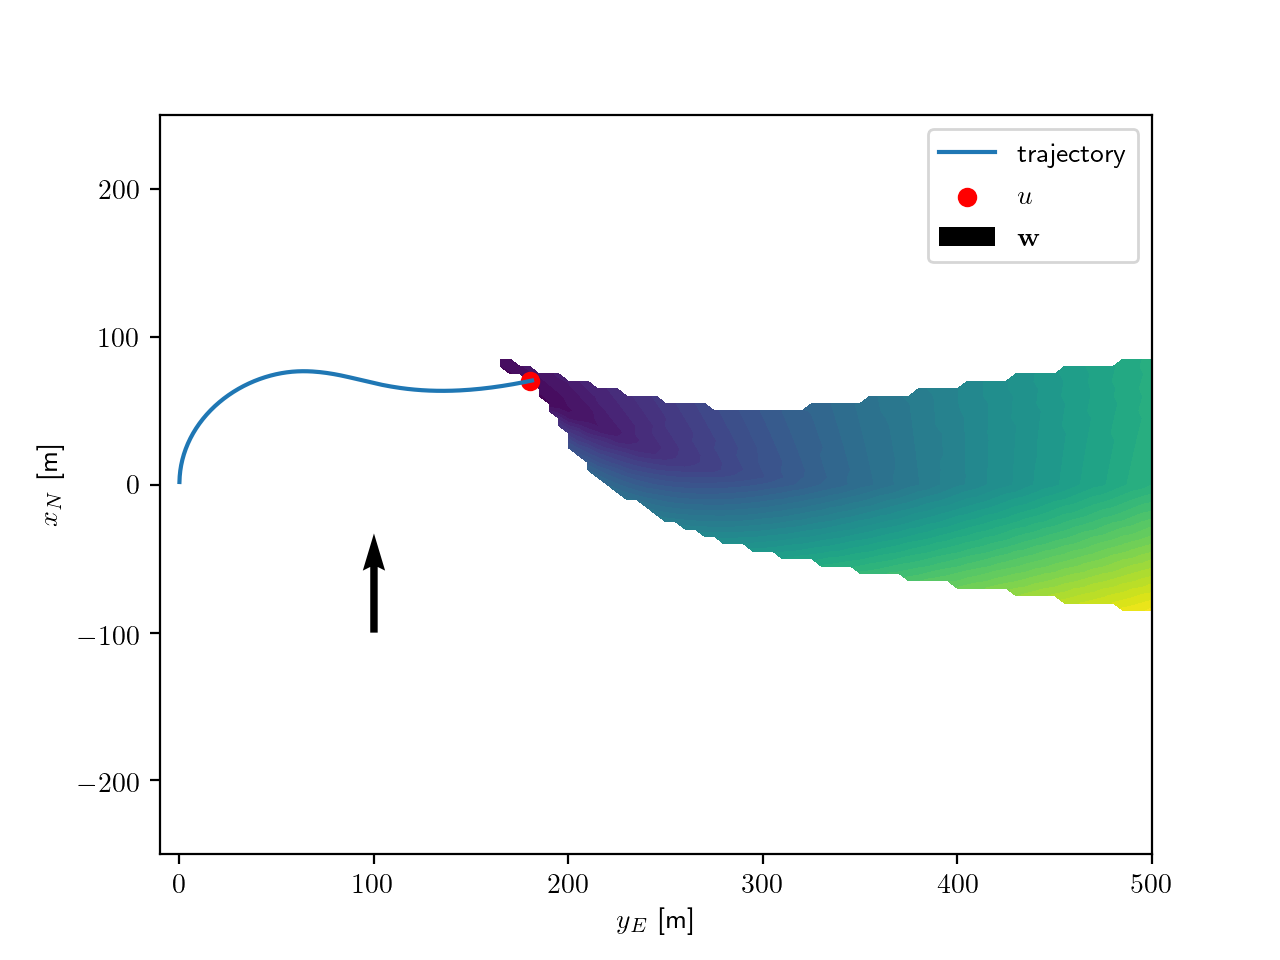
\includegraphics[width=.8\linewidth]{fig/J_opt_90.png}
        \end{center}
        \caption{$J$ for $\airspd=14$ m/s, $\windspd=5$ m/s, $\winddir=0\degree$, $\psi_d=90\degree$}
    \end{figure}
\end{frame}

\begin{frame}{Optimal control problem (contd)}
    Derivative free optimization methods

    \begin{subequations}
        \label{eq:derivative_free_opt}
        \begin{alignat}{3}
        &\min_{x\in\mathbb{R}^n}        &\qquad& f: x \rightarrow \mathbb{R} & \\
        &\text{subject to} & & x\in\states_{feasible} &\\
        \end{alignat}
    \end{subequations}

    Mesh-Adaptive Direct Search (\ac{MADS})
\end{frame}

\begin{frame}{Resulting primitives}
    \begin{figure}
        \begin{center}
            \subfloat[$\winddir=0\degree$]{
                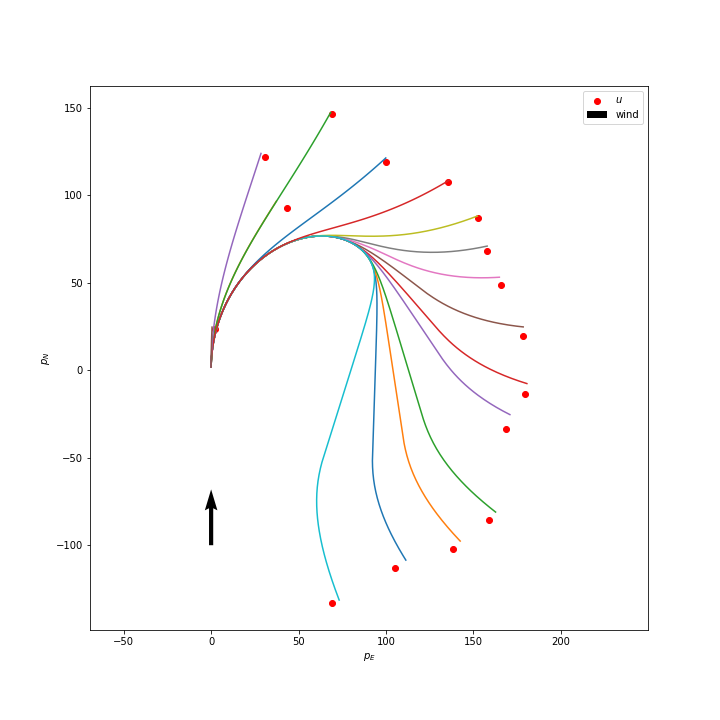
\includegraphics[width=.48\linewidth]{fig/mp_0}
            }
            \subfloat[$\winddir=80\degree$]{
                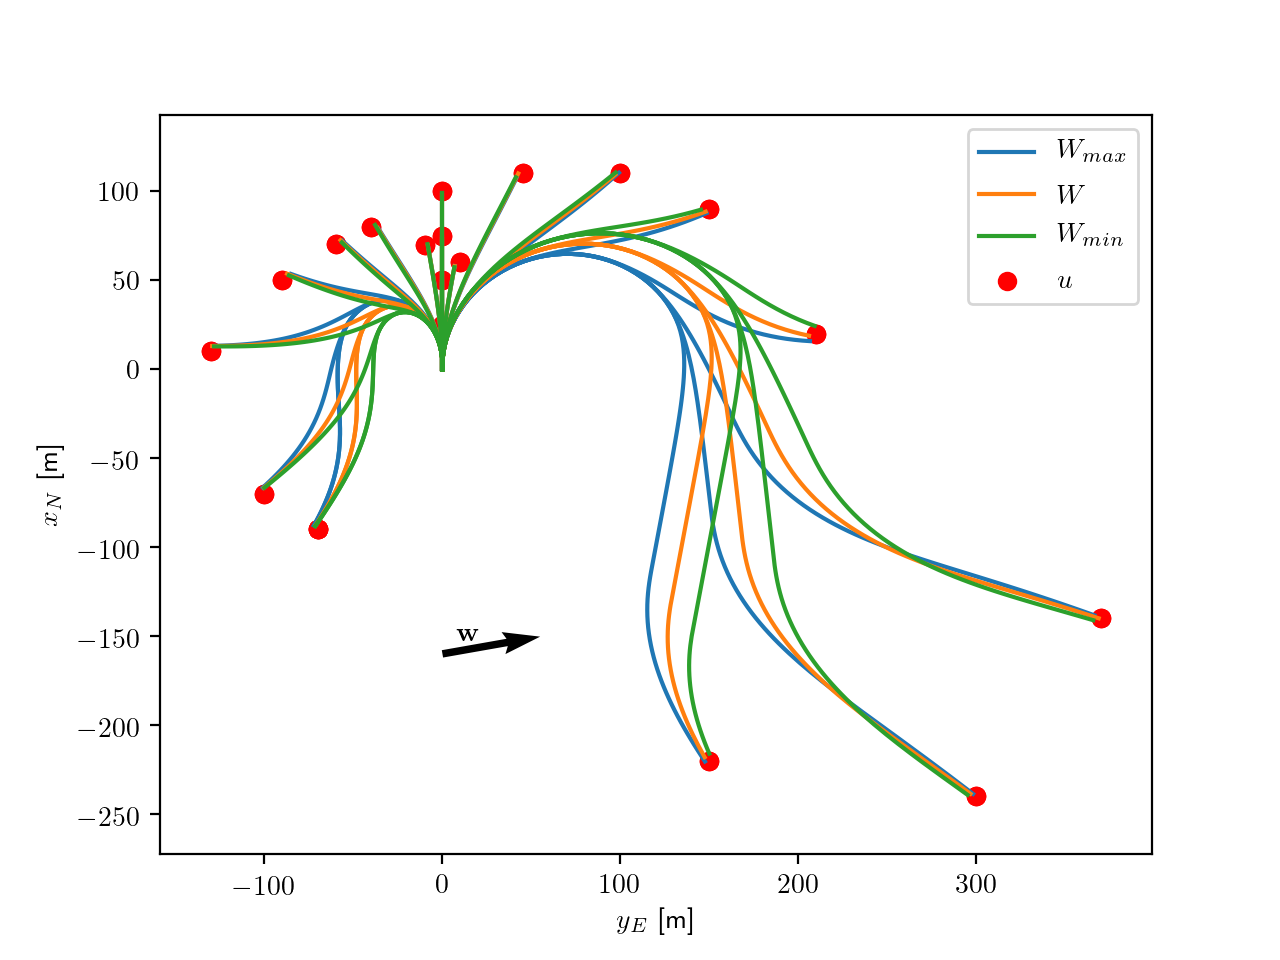
\includegraphics[width=.48\linewidth]{fig/mp_80}
            }
        \end{center}
        \caption{Motion primitives for different wind directions, $\windspd=5$ m/s}
        \label{fig:motion_prims}
    \end{figure}
\end{frame}

\begin{frame}{Heuristic function}
    \begin{itemize}
        \item States defined in inertial frame
        \item Cost is distance travelled by \ac{UAV} in air-relative frame
        \item Not equal to inertial frame distance if $\windspd\neq0$
    \end{itemize}
\end{frame}

\begin{frame}{Cost for straight line paths}
    Assuming that $\psi_i=\psi_f=\wca$:
    \begin{equation}
        V_{\parallel}=\cos\psi_s(\airspd\cos\wca+\windspd\cos\winddir) + \sin\psi_s(\airspd\sin\wca+\windspd\sin\winddir)
    \end{equation}
    \begin{equation}
        s_A=\frac{\airspd}{V_\parallel}\|\vec{p}_{i+1}-\vec{p}_{i}\|
    \end{equation}
\end{frame}

\begin{frame}{Cost for arbitrary initial and final heading}
    \begin{itemize}
        \item Dubin's path if $\windspd=0$
        \item No analytical solution if $\windspd\neq0$
        \item Numerical solutions exist but computationally expensive
    \end{itemize}
\end{frame}

\begin{frame}{Heuristic Look-Up Table}
    \begin{itemize}
        \item Entries for different values of $\psi_i$ from $0\degree$ to $180\degree$
        \item Different $\windspd$ require new HLUT
        \item Generated with Dijkstra's Algorithm using motion primitives
    \end{itemize}
\end{frame}

\begin{frame}{Heuristic Look-Up Table (contd)}
    \begin{figure}
        \begin{center}
            \resizebox{.5\linewidth}{!}{
                \begin{tikzpicture}
                    \draw (-2, -2) rectangle (2, 2);
        
                    \draw[my_v] (0,0) -- node[at end, below]{$y_E$} (1,0);
                    \draw[my_v] (0,0) -- node[at end, left]{$x_N$} (0,1);
        
                    \node[point] at (0,0){};
                    \node[below] at (0,0){$x$};
        
                    \node[point] at (2,1){};
                    \node[above] at (2,1){$x_p$};
                    \draw (0,0) -- node[midway, below, anchor=north west]{$h_{HLUT}(x, x_p)$} (2,1);
        
                    \node[point] at (4,2){};
                    \node[above] at (4,2){$x_g$};
                    \draw[dashed] (2,1) -- node[midway,below, anchor=north west]{$h_s(x_p,x_g)$} (4,2);
        
                    \node[anchor=west] at (-1.8,-1.75){HLUT available};
                \end{tikzpicture}
            }
        \end{center}
        \caption{Projection of queries on HLUT}
        \label{fig:hlut_proj}
    \end{figure}
\end{frame}

\begin{frame}{Heuristic Look-Up Table (contd)}
    \begin{figure}
        \begin{center}
            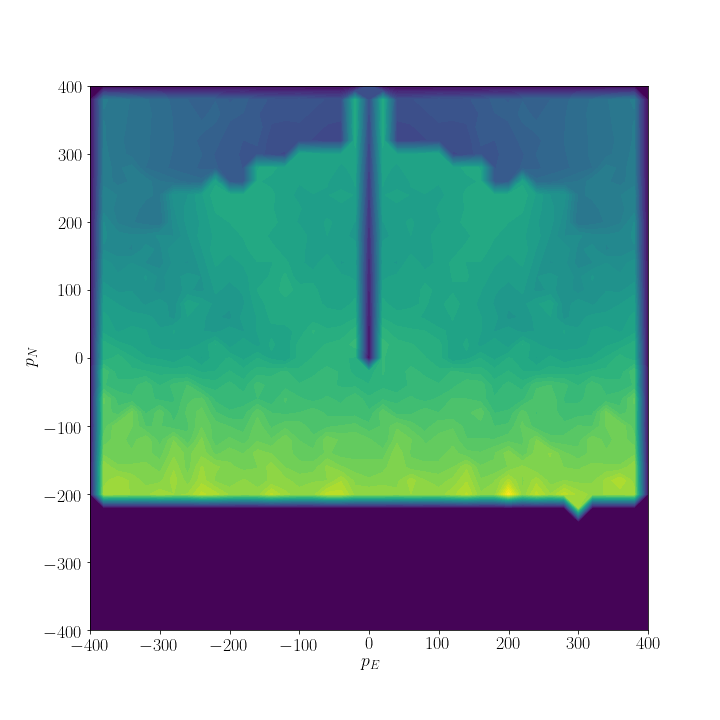
\includegraphics[width=.6\linewidth]{fig/hlut}
        \end{center}
        \caption{HLUT for $\psi_f=0\degree$}
    \end{figure}
\end{frame}

\section{Landing}
\begin{frame}{Landing sequences}
    \begin{figure}
        \begin{center}
            \resizebox{.8\linewidth}{!}{
                \begin{tikzpicture}
                    \coordinate (center) at ($(1,1)+(20:1.5)+(110:0.5)$);
                    \coordinate (a) at ($(center)+(-130:2)$);
                    \draw[fill=lightgray, rotate around={20:(1,1)}] (1,1) rectangle (4,2);
                    \draw[](0,1) -- ++ (80:1.5) -- ++ (20:1) -- ++ (45:0.75) -- (0,4) --++ (-2, -1.5) -- (-1,1) -- (0,1);
                    \node at (-.5,2.5){$\xobst$};
                    \node at ($(center)+(-160:1)$){$\landing$};
                    \draw (center) -- ++ (-130:2);
                    \node[point] at (center){};
                    \node[above] at (center){$\vec{p}_L$};
                    \node[point] at (a){};
                    \node[below] at (a){$\vec{p}_A$};
                    \draw[my_v] ($(center)+(20:3)$) -- node[above]{$\windvec$} ++ (-1,0);
                    \Drone{-1}{0}{10}
                    \draw[dashed](-1,0) -- (a);            
                \end{tikzpicture}
            }
        \end{center}
        \caption{Landing sequence definition}
        \label{fig:land}          
    \end{figure}
\end{frame}

\begin{frame}{Landing sequences (contd)}
    \begin{itemize}
        \item Approach: Descend at rate $\dot{h}$ given by $\vec{p}_A$ and $\vec{p}_L$
        \item Flare: When below altitude $\flarealt$, begin descending at fixed rate $\flaresink$
        \item Has to enter landing area $\landing$ above altitude $h_A$
    \end{itemize}
\end{frame}

\begin{frame}{Optimal landing sequence}
    Objectives:
    \begin{enumerate}
        \item Land as closely to the center of $\landing$ as possible
        \item Land against the wind if possible
    \end{enumerate}
\end{frame}

\begin{frame}{Optimal landing sequence (contd)}
    \begin{figure}
        \begin{center}
            \resizebox{.6\linewidth}{!}{
                \begin{tikzpicture}
                    \coordinate (center) at (2,1);
                    \coordinate (p1) at ($(center)+(-1.5,-1)$);
                    \coordinate (p2) at ($(center)+(1.5,1)$);
                    \coordinate (pa) at ($(p1)+(-.75,-.5)$);
                    \coordinate (pl) at ($(center)+(.75,.5)$);
        
                    \draw[fill=lightgray] (0,0) rectangle (4,2);
                    \node[point] at (p1){};
                    \node[below] at (p1){$\vec{p}_1$};
        
                    \node[point] at (p2){};
                    \node[above] at (p2){$\vec{p}_2$};
        
                    \node[point] at (center){};
                    \node[above] at (center){$\vec{p}_c$};
        
                    \draw[dashed] ($(p1)+(-3,-2)$) -- (p2);
                    \node[below] at (pa){$\vec{p}_A$};
                    \node[point] at (pa){};
        
                    \node[above] at (pl){${\vec{p}_L}$};
                    \node[point] at (pl){};
        
                    \draw[line width=1.5pt] (pa) -- (pl);
        
                    \Drone{-2.5}{-2}{30};
                    \draw[dashed] ($(-2.5,-2)+(.75,.5)$) -- ++ (1,0);
                    \draw ($(-2.5,-2)+(1.25,.5)$) arc(0:30:.5) node[midway, anchor=200]{$\psi_L$};
        
                    \node at (3.5,.5){$\landing$};
                    \draw[my_v] (2, 4) -- node[left]{$\windvec$} ++ (0,-1);
                \end{tikzpicture}
            }
        \end{center}
        \caption{Variables to determine optimal landing sequence}
        \label{fig:opt_landing}
    \end{figure}
\end{frame}

\begin{frame}{Optimal landing sequence (contd)}
    Divided into two steps:
    \begin{enumerate}
        \item Determine $\psi_L$
        \item Determine $R_a=\|\vec{p}_A-\vec{p}_2\|$ and $R_l=\|\vec{p}_L-\vec{p}_2\|$
    \end{enumerate}
\end{frame}

\begin{frame}{Determining approach direction}
    \begin{equation}
        V_L(\psi)=\cos\psi(\airspd\cos\wca+\windspd\cos\winddir) + \sin\psi(\airspd\sin\wca+\windspd\sin\winddir)
    \end{equation}
    \begin{equation}
        R_{\text{min}}(\psi)=V_L(\psi)\frac{h_A-\flarealt}{\dot{h}_{\text{max}}}
    \end{equation}
    \begin{equation}
        R_{flare}(\psi)=V_{L}(\psi)\frac{\flarealt}{\flaresink}
    \end{equation}
\end{frame}

\begin{frame}{Determining approach direction (contd)}
    $L(\psi)$: Line from $\vec{p}_1$ in direction $\psi+180\degree$ with length $K$ for some $K\geq0$
    \begin{equation}
        \{\psi_L\}_{feas}=\{\psi: (R(\psi)\geq R_{\text{min}}(\psi)+R_{flare}(\psi)) \cap (L(\psi)\notin \xobst)\}
    \end{equation}
    \begin{equation}
        \psi_{L,opt} = \argmin_{\psi\in\{\psi_{L}\}_{feas}}R(\psi)
    \end{equation}
\end{frame}

\begin{frame}{Determining approach parameters}
    \begin{equation}
        \dot{h} = f(R_a, R_l)
    \end{equation}
    \begin{equation}
        h(R) = h_0 - R\frac{\dot{h}}{V_L}
    \end{equation}
    \begin{equation}
        R_c = \|\vec{p_1}-\vec{p}_2\|
    \end{equation}
\end{frame}

\begin{frame}{Determining approach parameters (contd)}
    Constraints:
    \begin{equation}\label{eq:h_a_constraint}
        h(R_a - 2R_c) \geq h_A
    \end{equation}
    \begin{equation}\label{eq:h_f_constraint}
        h(R_a - R_{flare} - R_l) = \flarealt
    \end{equation}
\end{frame}

\begin{frame}{Determining approach parameters (contd)}
    \begin{subequations}
        \label{eq:opt_problem_land}
        \begin{alignat}{3}
        &\min_{R_a,R_l}        &\qquad& J=R_a^2 + \lambda|R_c-R_l|^2 & \\
        &\text{subject to} & & R_a,R_l\geq0 &\\
        & & & \dot{h}(R_a, R_l)\leq \dot{h}_{\text{max}}\\
        & & & \eqref{eq:h_a_constraint} \nonumber\\
        & & & \eqref{eq:h_f_constraint} \nonumber
        \end{alignat}
    \end{subequations}
\end{frame}

\begin{frame}{System overview}
    \begin{figure}
        \begin{center}
            \resizebox{.8\linewidth}{!}{
                \begin{tikzpicture}[node distance = 3cm, auto]
                    \node[block] (init){Landing area input};
                    \node[block, right of=init] (land){Landing sequence calculation};
                    \node[block, below of=land] (obst){Obstacle database};
                    \node[block, above of=land] (wind){Wind estimation};
                    \node[block, right of=land] (mp){Motion planner};
                    \node[block, above of=mp] (gps){Positioning system};
                    \node[block, right of=mp] (traj){Waypoint controller};
        
                    \path[line] (init) - > node{$\landing$} (land); 
                    \path[line] (obst) - > node[midway, right]{$\xobst$} (land);
                    \path[line] (obst) - > node[midway, right]{$\xobst$} (mp);
                    \path[line] (wind) - > node[midway, right]{$\windvec$} (land);
                    \path[line] (wind) - > node[midway, right]{$\windvec$} (mp);
                    \path[line] (land) - > node[midway]{$x_g$} (mp);
                    \path[line] (gps) - > node[midway, right]{$x_0$} (mp);
                    \path[line] (mp) - > node[midway]{$\mathcal{M}$} (traj);
                \end{tikzpicture}
            }
        \end{center}
        \caption{System overview}
        \label{fig:sys_overview}
    \end{figure}
\end{frame}

\begin{frame}{Results}
    \begin{figure}
    
        \subfloat[$\winddir=0\degree$]{
            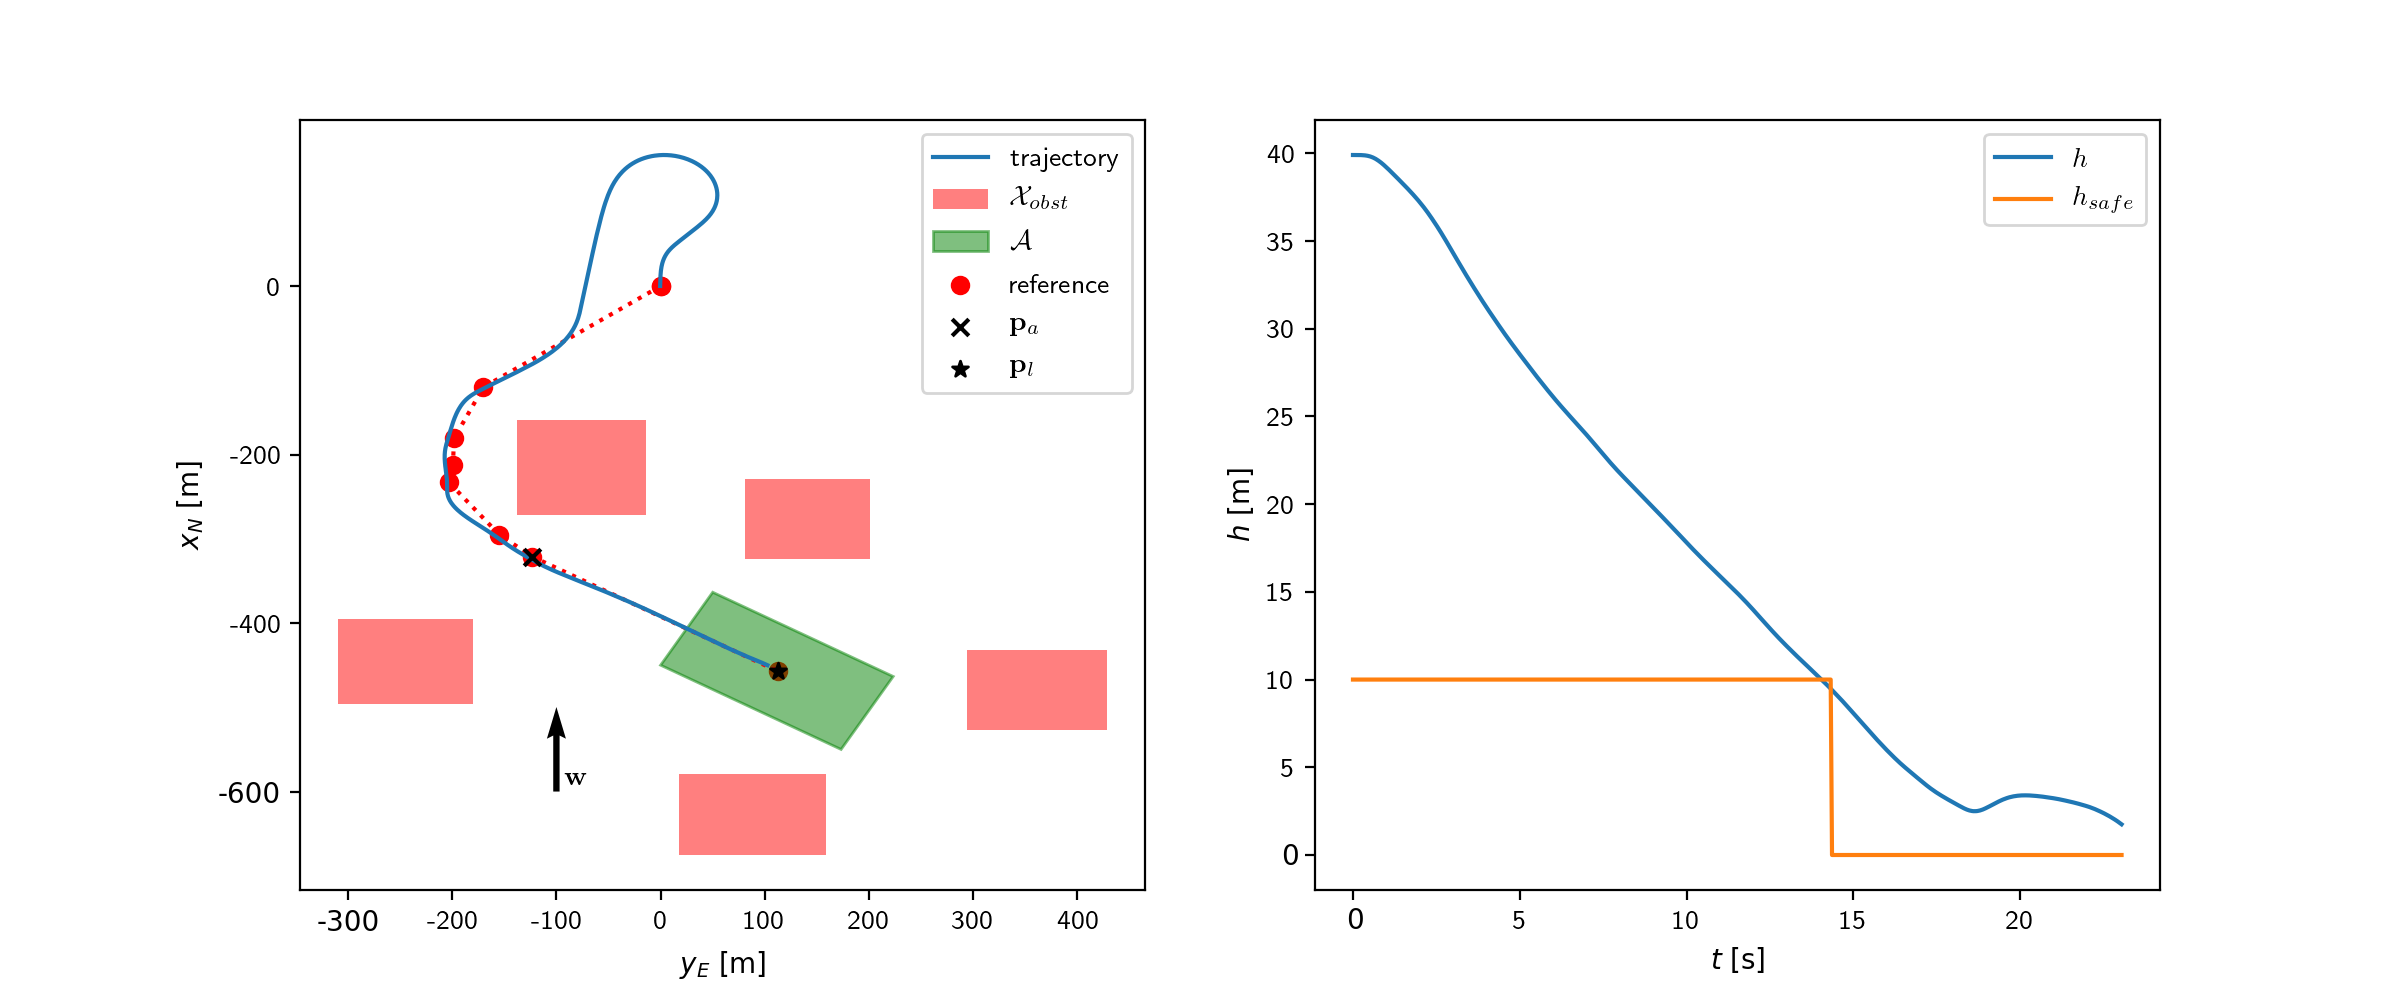
\includegraphics[width=.48\linewidth]{fig/sol_0}
        }
        \subfloat[$\winddir=90\degree$]{
            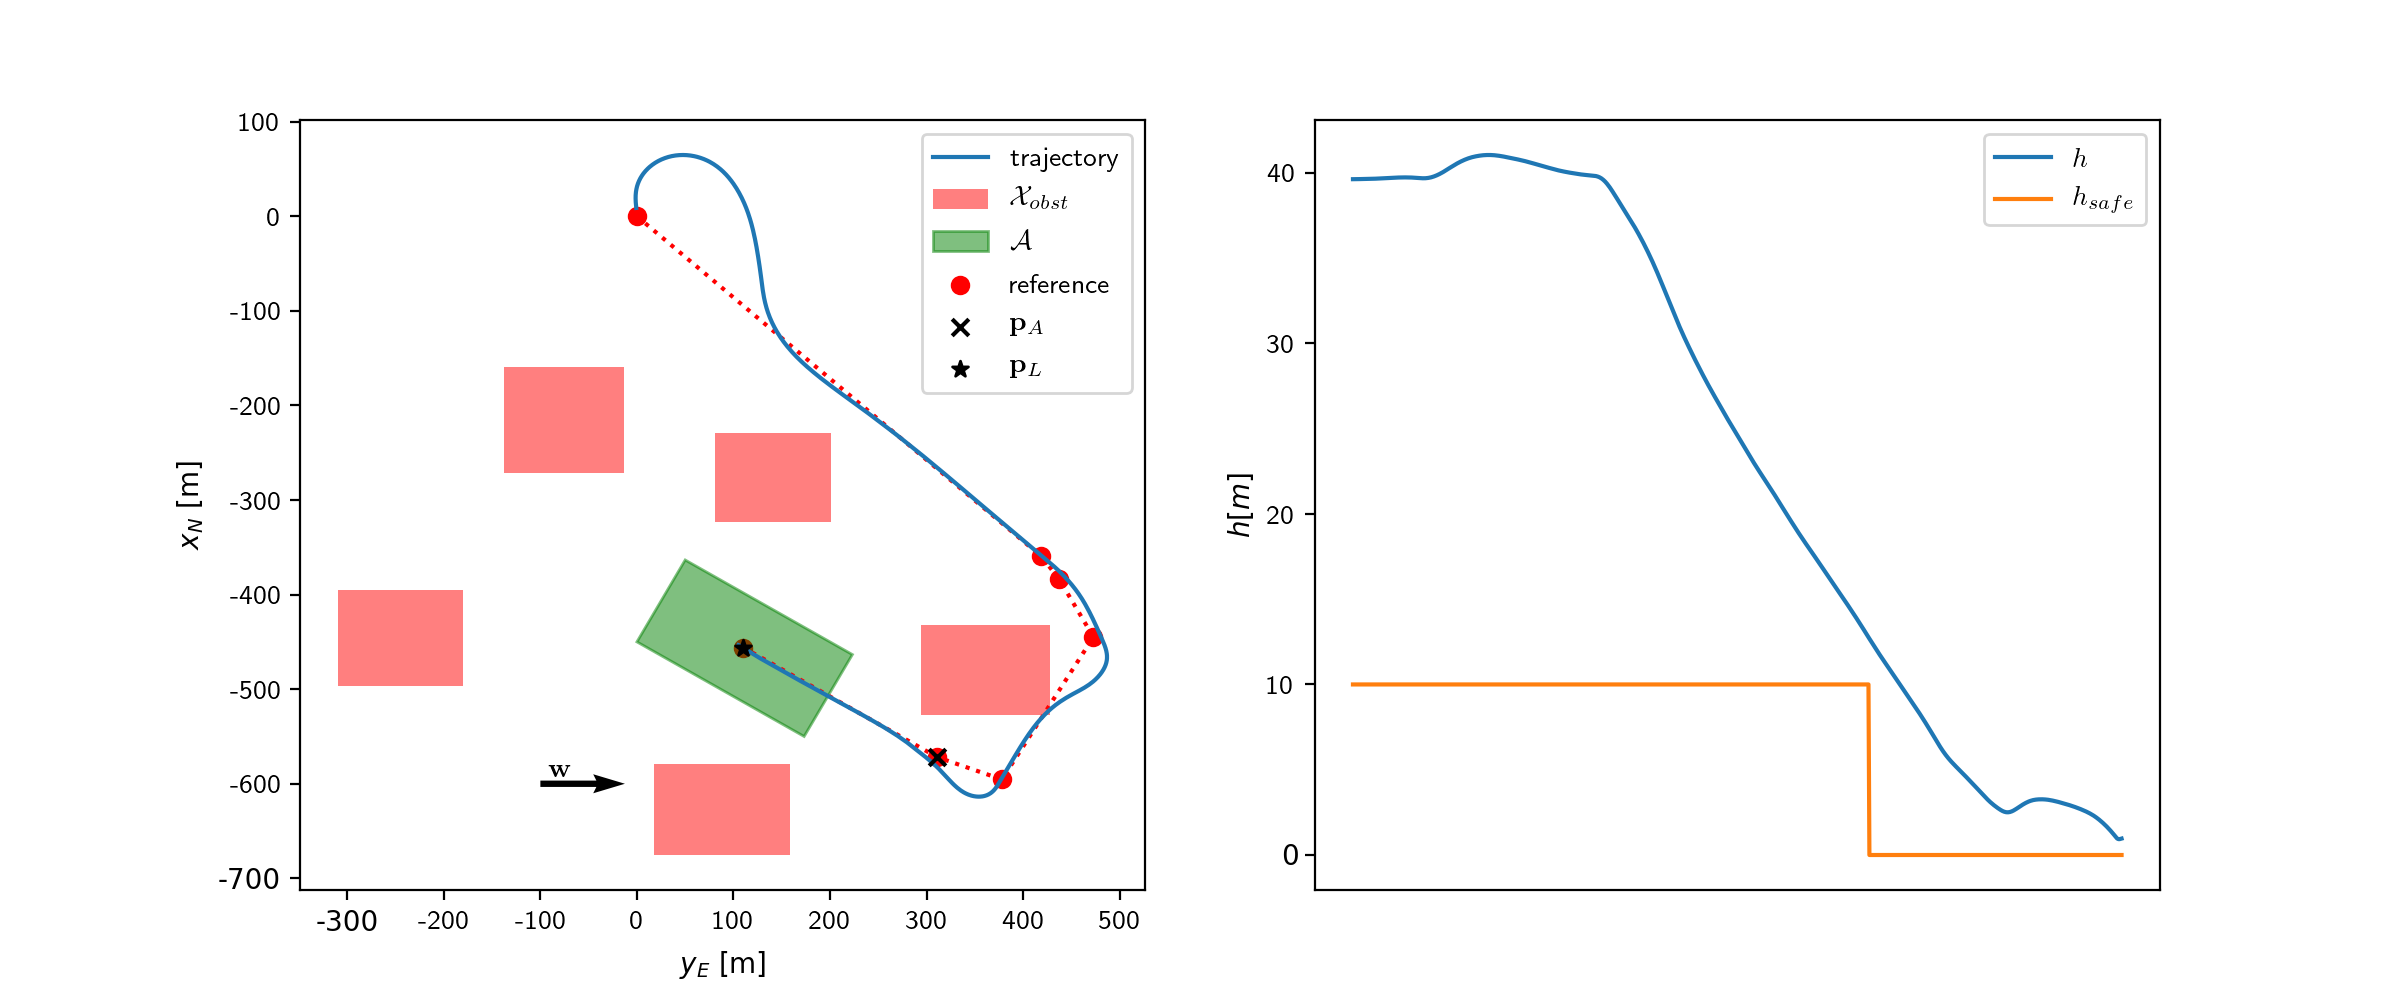
\includegraphics[width=.48\linewidth]{fig/sol_90}
        }
        \caption{Resulting landing procedures for different wind directions, $\windspd=5$ m/s}
        \label{fig:result}
    \end{figure}
\end{frame}

\begin{frame}{Results (contd)}
    \begin{figure}
    
        \subfloat[$\winddir=0\degree$]{
            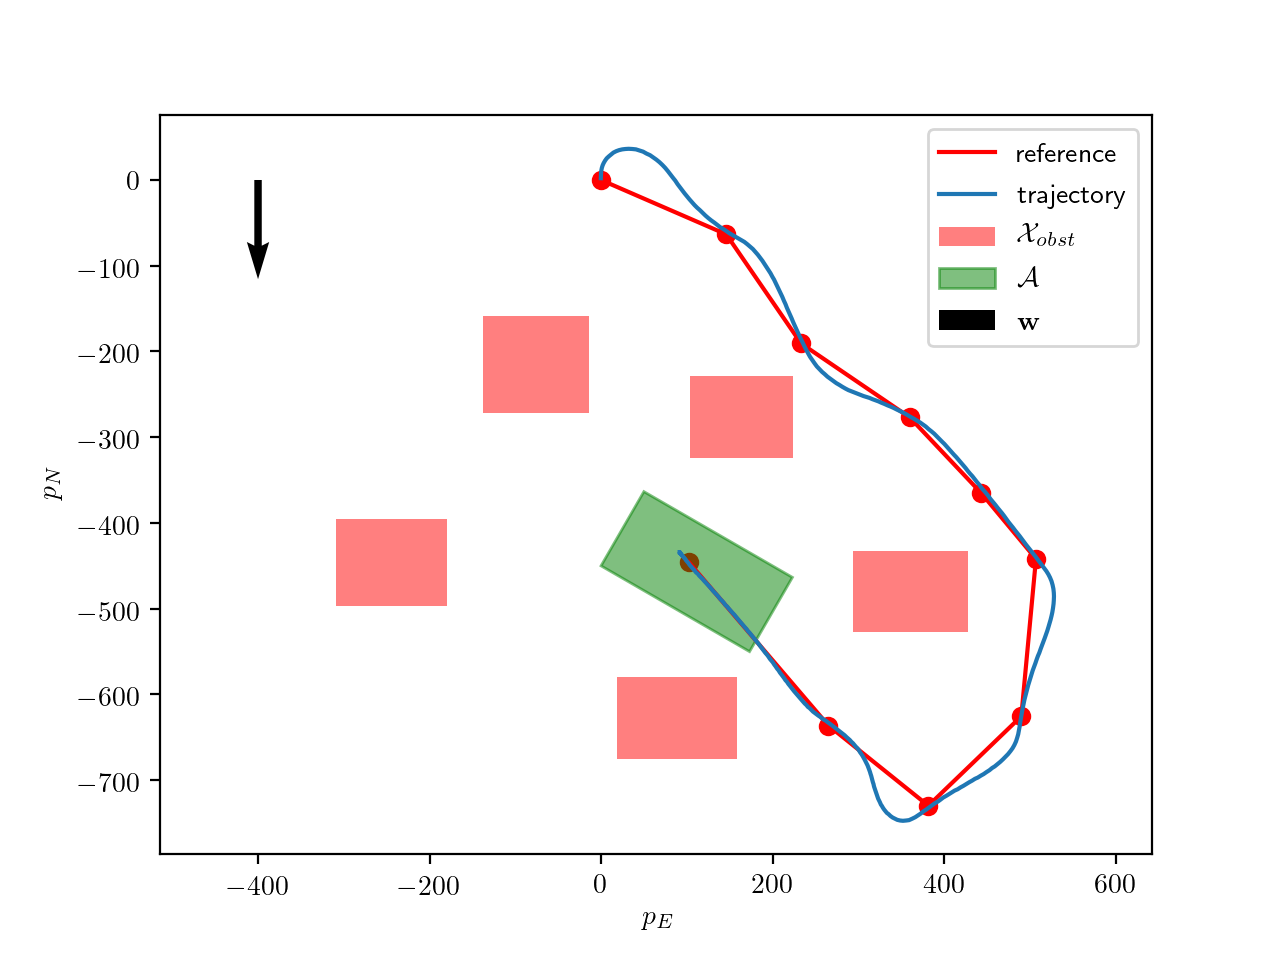
\includegraphics[width=.48\linewidth]{fig/sol_180}
        }
        \subfloat[$\winddir=90\degree$]{
            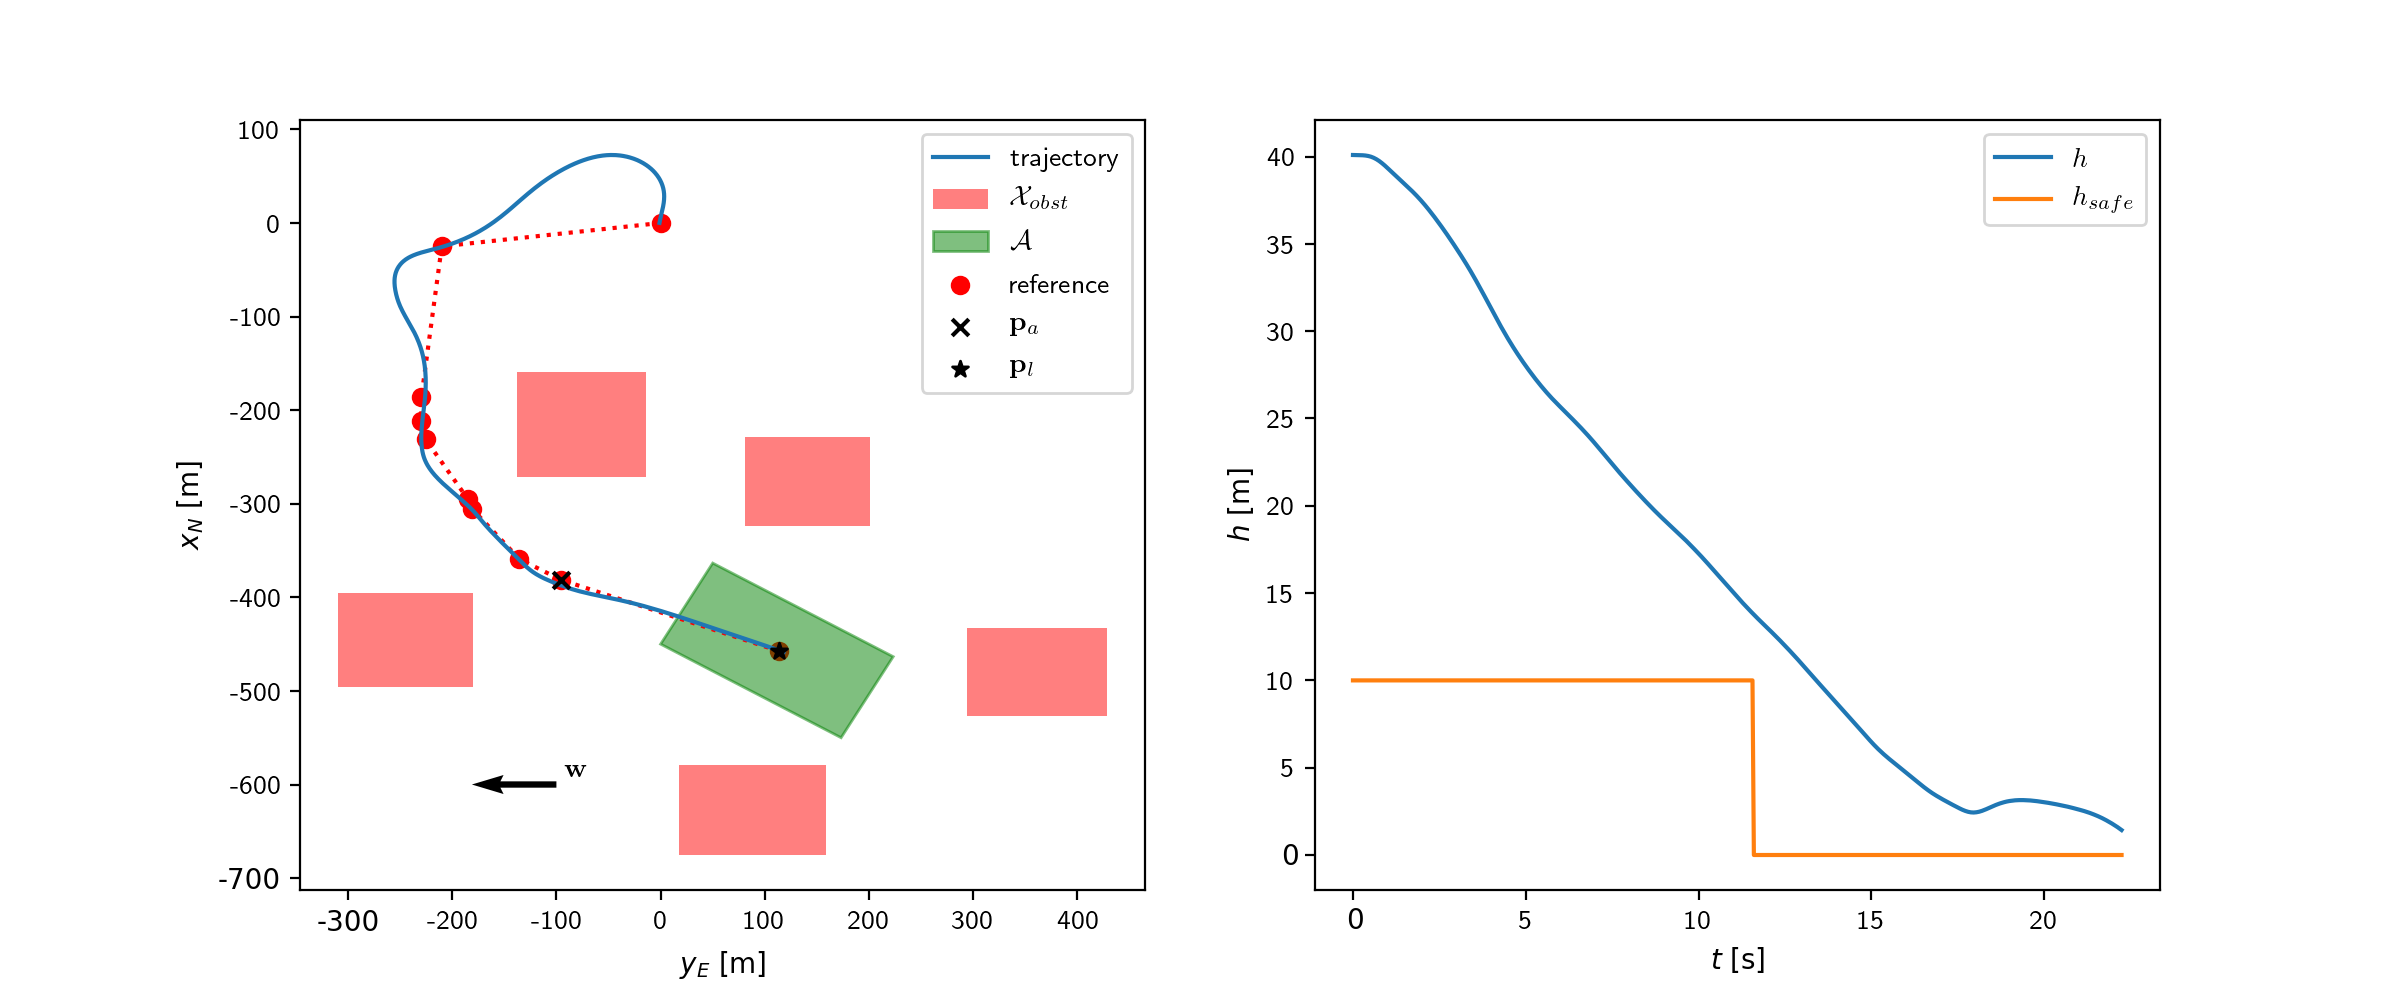
\includegraphics[width=.48\linewidth]{fig/sol_270}
        }
        \caption{Resulting landing procedures for different wind directions, $\windspd=5$ m/s}
        \label{fig:result}
    \end{figure}
\end{frame}

\begin{frame}{Possible improvements}

\begin{itemize}
    \item Extend formulation to handle varying winds with the same motion primitive set/HLUT 
    \item Investigate admissibility of heuristic (especially projection)
    \item Handle wind variations in landing sequence generation
    \item Estimate wind mean and variance online from measurements
\end{itemize}
    
\end{frame}

\end{document}